\subsection{Cruces ferroviarios}

\begin{algorithm}[hbt!]
        \caption{Level crossing algorithm}\label{alg:LC}
        \DontPrintSemicolon
        %\SetAlgoLined
        \SetNoFillComment
        \LinesNotNumbered 
        \For { netElement WITH LevelCrossing }
        {
            \tcc{Before reaching level crossing}
            [Signals] $\gets$ ADD circulation signal $>>>$\;
            \tcc{After leaving level crossing}
            [Signals] $\gets$ ADD circulation signal $<<<$\;
        }
        \KwResult{[Signals]} 
    \end{algorithm}
    
Los cruces ferroviarios son la intersección entre la vía ferroviaria y una ruta vehicular o peatonal. Estos cruces pueden ser bajo nivel (túnel por debajo de la vía), sobre nivel (puente vehicular por sobre la vía) o a nivel. Un paso a nivel es una zona muy crítica del sistema ferroviario, ya que, a diferencia de un paso sobre nivel o bajo nivel, conviven simultáneamente la formación y el transito vehicular y peatonal. En la Figura \ref{fig:cruce_1} se ilustra la intersección entre el tendido ferroviario, un cruce vehicular y un cruce peatonal.

    \begin{figure}[!h]
        \centering
        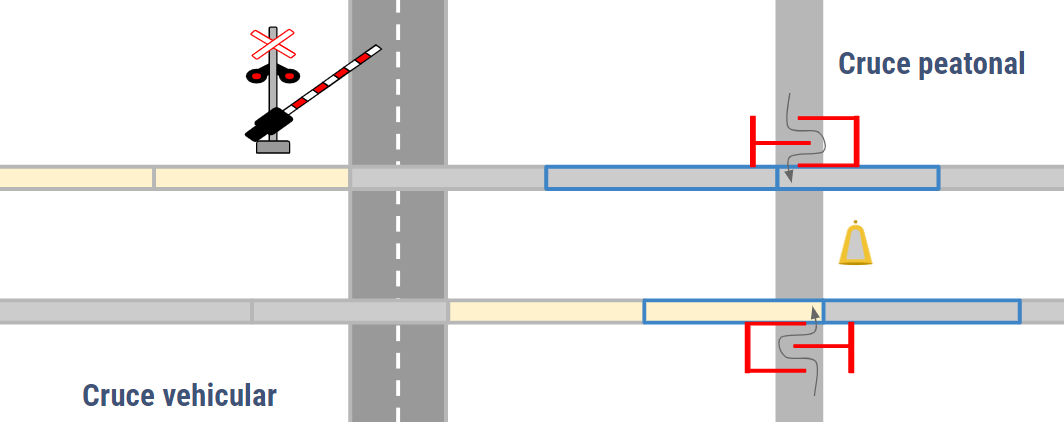
\includegraphics[width=1\textwidth]{Figuras/cruce}
        \centering\caption{XXXXX.}
        \label{fig:cruce_1}
    \end{figure}
    
Los pasos a nivel peatonales incluyen un pequeño laberinto zigzagueante para forzar al peatón a aminorar su marcha y ver a ambos lados antes de cruzar las vías. A menudo suelen estar acompañados de indicaciones lumínicas y sonoras que se accionan tan pronto el tren se encuentre dentro de un rango de varios metros cercano al paso a nivel.

Los pasos a nivel vehiculares añaden barreras ferroviarias para detener el tráfico vehicular cuando un tren se encuentra dentro de un rango de seguridad definido.  El sistema de control de la barrera mantiene el brazo de esta en alto para permitir la circulación vehicular. Si un tren es detectado cerca del paso a nivel, se desenergiza la barrera y comienza a descender el brazo por efecto de la gravedad. Solo cuando la barrera baja, el tren tiene permitido avanzar sobre el cruce, siendo el paso a nivel un sector de altísimo riesgo. Al desocuparse las secciones próximas al paso a nivel, la barrera vuelve a energizarse y se sitúa en estado alto nuevamente, a la espera de otro tren para reiniciar el proceso. 

Se debe destacar que el mismo proceso de descenso de la barrera ocurrirá si esta se desenergiza por una falla electricomecánica y/o pérdida de alimentación. Es decir, el sistema asumirá el estado más seguro ante cualquiera de los mencionados fallos, siguiendo el principio de falla segura.